\documentclass[11pt, letterpaper]{article}
\usepackage[utf8]{inputenc}
\usepackage[spanish]{babel}
\usepackage[margin=0.75in,top=1in,bottom=1in]{geometry}
\usepackage{amsmath}
\usepackage{lipsum}
\usepackage{csquotes}
\usepackage{float}
\usepackage[backend=biber,style=ieee]{biblatex}
    \addbibresource{biblio.bib}
\usepackage{hyperref}
    \hypersetup{%
    colorlinks=true,
    linkcolor=black,
    urlcolor=blue,
    citecolor=blue}
\usepackage{ragged2e}
\usepackage{graphicx}
\usepackage{adjustbox}
\usepackage[font=footnotesize,labelfont=bf]{caption}
\usepackage{subcaption}
\usepackage{dirtytalk}
\usepackage[table,xcdraw]{xcolor}
\usepackage{booktabs}
\usepackage{listings}
    \NewDocumentCommand{\codeword}{v}{%
    \texttt{\textcolor{orange}{#1}}%
    }
    \lstset{language=C,keywordstyle={\bfseries \color{orange}}}
\usepackage{tabularx}
    \newcolumntype{R}{>{\raggedleft\arraybackslash}X}
    \newcolumntype{Y}{>{\centering\arraybackslash}X}
%\usepackage{kpfonts}
\usepackage{cleveref}
\usepackage{parskip}

\captionsetup[subfigure]{subrefformat=simple,labelformat=simple}
\renewcommand\thesubfigure{(\alph{subfigure})}

\begin{document}

% Página de portada ----
\begin{titlepage}
\begin{center}


\includegraphics[height=10cm]{figuras/Logo-ITESO-Vertical (HQ).png}
    
\vspace{1in}

\textbf{{\large Proyecto 02}}\\ \vspace{0.25cm}
\textbf{{\Huge Boston Housing}}\\ \vspace{0.5cm}
Minería de Datos --- Primavera 2022\\
ESI3466K\\
\today \\ 
    
\vspace{0.5cm}
    
\begin{tabularx}{0.9\linewidth}{YY}
OLVERA HERNÁNDEZ, ROEBRTO & ib721045\\
\textbf{Profesor:} & Dr. Juan Antonio Vega Fernández
\end{tabularx}
    
\vspace{0.5in}
    
Instituto Tecnológico y de Estudios Superiores de Occidente (ITESO)\\
\end{center}

\begin{flushright}
{\small San Pedro Tlaquepaque, Jalisco, MX.}
\end{flushright}

\newpage
\end{titlepage}
% ----------------------

\tableofcontents\newpage

\section{Introducción}
\subsection{El dataset \textit{Boston Housing}}
El conjunto de datos \textit{Boston Housing} fue publicado originalmente por \textcite{Harrison1978} en 1978, tomando datos publicados por el Servicio de Censo Poblacional de los Estados Unidos (U.S CS) de la ciudad de Boston, MA. 

Inicialmente se publicó el artículo con el objetivo de evaluar el precio de la vivienda en la ciudad en función de la calidad del aire utilizando solo dos variables. Actualmente, la estructura del set constituye de 506 observaciones o \textit{casos} (filas) con 14 variables (columnas), ver Cuadro \ref{tab:variables}, y es utilizando en gran medida como caso de estudio para \textit{aprendizaje estadístico} \cite{al2018comparative, shahhosseini2019optimizing, lin2008particle, ryffel2018generic, timofeev2004classification}.


\subsection{Regresión lineal múltiple}
Asumimos el  siguiente modelo:
\begin{equation}
    Y = \beta_0 + \beta_1 X_1 + \beta_2 X_2 + \ldots + \beta_p X_p + \epsilon
\end{equation}
donde las variables $\beta_0$ y $\beta_1$ son constantes desconocidas que representan el \textit{intercepto} y la \textit{pendiente}, respectivamente, también conocidos como \textit{coeficientes} o \textit{parámetros}, y $\epsilon$ es el error.

Dadas las estimaciones $\hat{\beta_0}$ y $\hat{\beta_1}$ para los coeficientes del modelo, podemos predecir valores futuros en una cantidad $i$ de variables con:

\begin{equation}
    \hat{y} = \beta_0 + \beta_1 \hat{x}_1+ \beta_2 \hat{x}_2 + \ldots + \beta_i \hat{x}_i
\end{equation}

donde $\hat{y}$ indica una predicción\footnote{El \textit{circunflejo} representa valores estimados.} $Y$ respecto a $X=x$.

Sea $\hat{y_i} = \beta_0 + \beta_1 \hat{x_i}$ la predicción $Y$ basado en el valor $i$-ésimo del valor $X$. Después, dado el error $e_i = y_i - \hat{y}_i$ podemos definir la \textit{Suma Residual de Cuadrados} (RSS, por sus siglas en inglés):

\begin{equation}
    \mathrm{RSS} = \sum_{n}^{i=1} (y_i - \hat{\beta}_0 - \hat{\beta}_{1} x_{i1} - \hat{\beta}_{2} x_{i2} - \ldots - \hat{\beta}_{p} x_{ip})^2
\end{equation}

La aproximación de mínimos cuadrados usa $\hat{\beta}_0$ y $\hat{\beta}_1$ para minimizar la RSS. Minimizando los valores se puede mostrar que:
\begin{equation}
    \hat{\beta}_1 = \frac{ \sum_{i=1}^{n} (x_i - \bar{x})(y_i - \bar{y}) }{ \sum_{i=1}^{n} (x_i - \bar{x})^2 }
\end{equation}
donde $\bar{y} \equiv \frac{1}{n}\sum_{i=1}^{n} y_i$ y $\bar{x} \equiv \frac{1}{n}\sum_{i=1}^{n} x_i$ son las medias de los datos.

Para evaluar la \textbf{precisión general} del modelo de regresión lineal se pueden calcular 3 medidas del error: 1) \textit{Error Estándar de Residuales} (Ec. \ref{eq:rse}); 2) \textit{R-cuadrada} (Ec. \ref{eq:r2}); y 3) \textit{Suma Total de Cuadrados} (Ec. \ref{eq:r}):

\begin{equation}
    \mathrm{RSE} = \sqrt{\frac{1}{n-2}\mathrm{RSS}} = 
    \sqrt{\frac{1}{n-2} \sum_{i=i}^{n} (y_i - \hat{y}_i)^2 }
    \label{eq:rse}
\end{equation}

\begin{equation}
    \mathrm{R^2} = 1-\mathrm{\frac{RSS}{TSS}} = 
    1 - \frac{\sum_{i=1}^{n} (y_i - \hat{y}_i)^2 }{\sum_{i=1}^{n} (y_i - \bar{y})^2}
    \label{eq:r2}
\end{equation}

\begin{equation}
    r = \frac{ \sum_{i=1}^{n} (x_i - \bar{x})(y_i - \bar{y}) }{
    \sqrt{ \sum_{i=1}^{n} (x_i - \bar{x})^2 }
    \cdot
    \sqrt{ \sum_{i=1}^{n} (y_i - \bar{y})^2 }
    }
    \label{eq:r}
\end{equation}

\section{Metodología}

Todo el análisis de datos fue realizado usando la plataforma \codeword{Orange} con el flujo de trabajo que se muestra en la Figura \ref{fig:workflow}.

\begin{figure}[htb!]
	\centering
    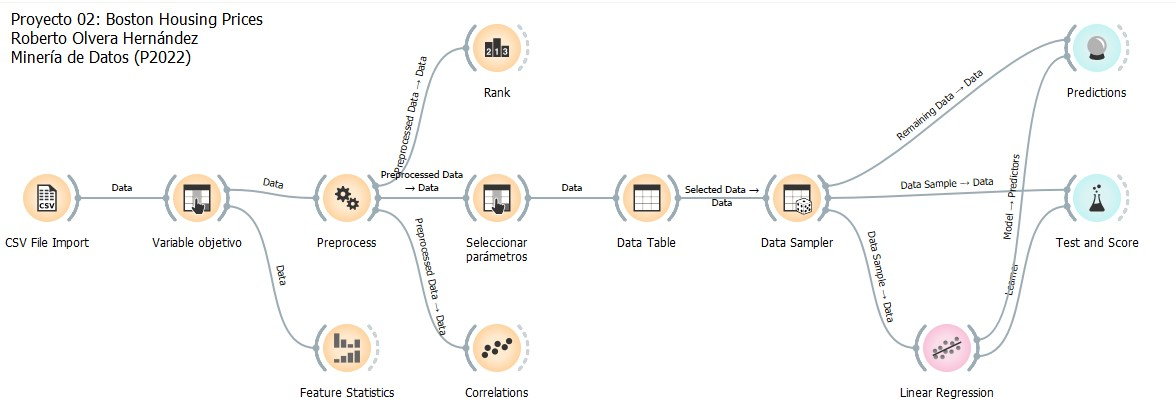
\includegraphics[width=0.95\textwidth]{figuras/orange workflow.jpg}
	\caption{Flujo de trabajo de Modelo Lineal Mútltiple.}
	\label{fig:workflow}
\end{figure}

\subsection{Preprocesamiento de datos}
Antes de realizar cualquier arreglo en el conjunto de datos, se definió que la variable \codeword{CHAS} sería \textit{categórica} en vez de una \textit{numérica} como se detecta originalmente, ya que son números nominales que indican valores \codeword{TRUE} o \codeword{FALSE} con 0 y 1. Una vez redefinida, se utilizó el widget \codeword{Preprocess} para normalizar los datos en un intervalo [0,1] y eliminar valores \textit{nulos}.

En seguida, se seleccionaron las 5 variables con mejor puntuación para obtener mayor información sobre \codeword{MEDV} según el widget \codeword{Rank}. Las variables fueron: 1) LSTAT; 2) RM; 3) PTRATIO; 4) AGE; 5) NOX. Estas se mandaron después a un \codeword{Data Table} y finalmente con el widget \codeword{Data Sampler} se seleccionaron el 70\% y 30\% de los datos para mandarlos al modelo de RLM y el predictor, respectivamente.

\subsection{Regresión lineal múltiple}
Una vez limpiados los datos, se corrieron las 6 variables en el widget de \codeword{Linear regression} sin regularizaciones con el 70\% de los datos obtenidos con el widget anterior y evaluados con \codeword{Test \& Score}. El resto de los datos se enviaron a \codeword{Predictions}.

\section{Resultados y discusión}
\subsection{Exploración general de los datos}
Un gráfico de cajas y bigotes (Figura \ref{fig:descriptive}(a)) muestra que la tasa de criminalidad (\codeword{CRIM}) es extremadamente baja, la mayoría cercanos al 0\%, también hay bastantes \textit{outliers} que pueden ser identificados. También podemos observar que muy pocas zonas residenciales tienen lotes mayores a 25,000$\mathrm{ft}^2$ (\codeword{ZN}).

Otra característica interesante que se encuentra en valores extremos es la proporción de personas negras (\codeword{B}). Hay que tomar en cuenta que la función $1000\cdot (B_k - 0.63)^2 \propto B_k$, así, podemos observar que en la mayoría de las zonas residenciales cuentan con una población mayormente negra ($65.94\pm 0.56$\%). 

\begin{figure}[htb!]
	\centering
	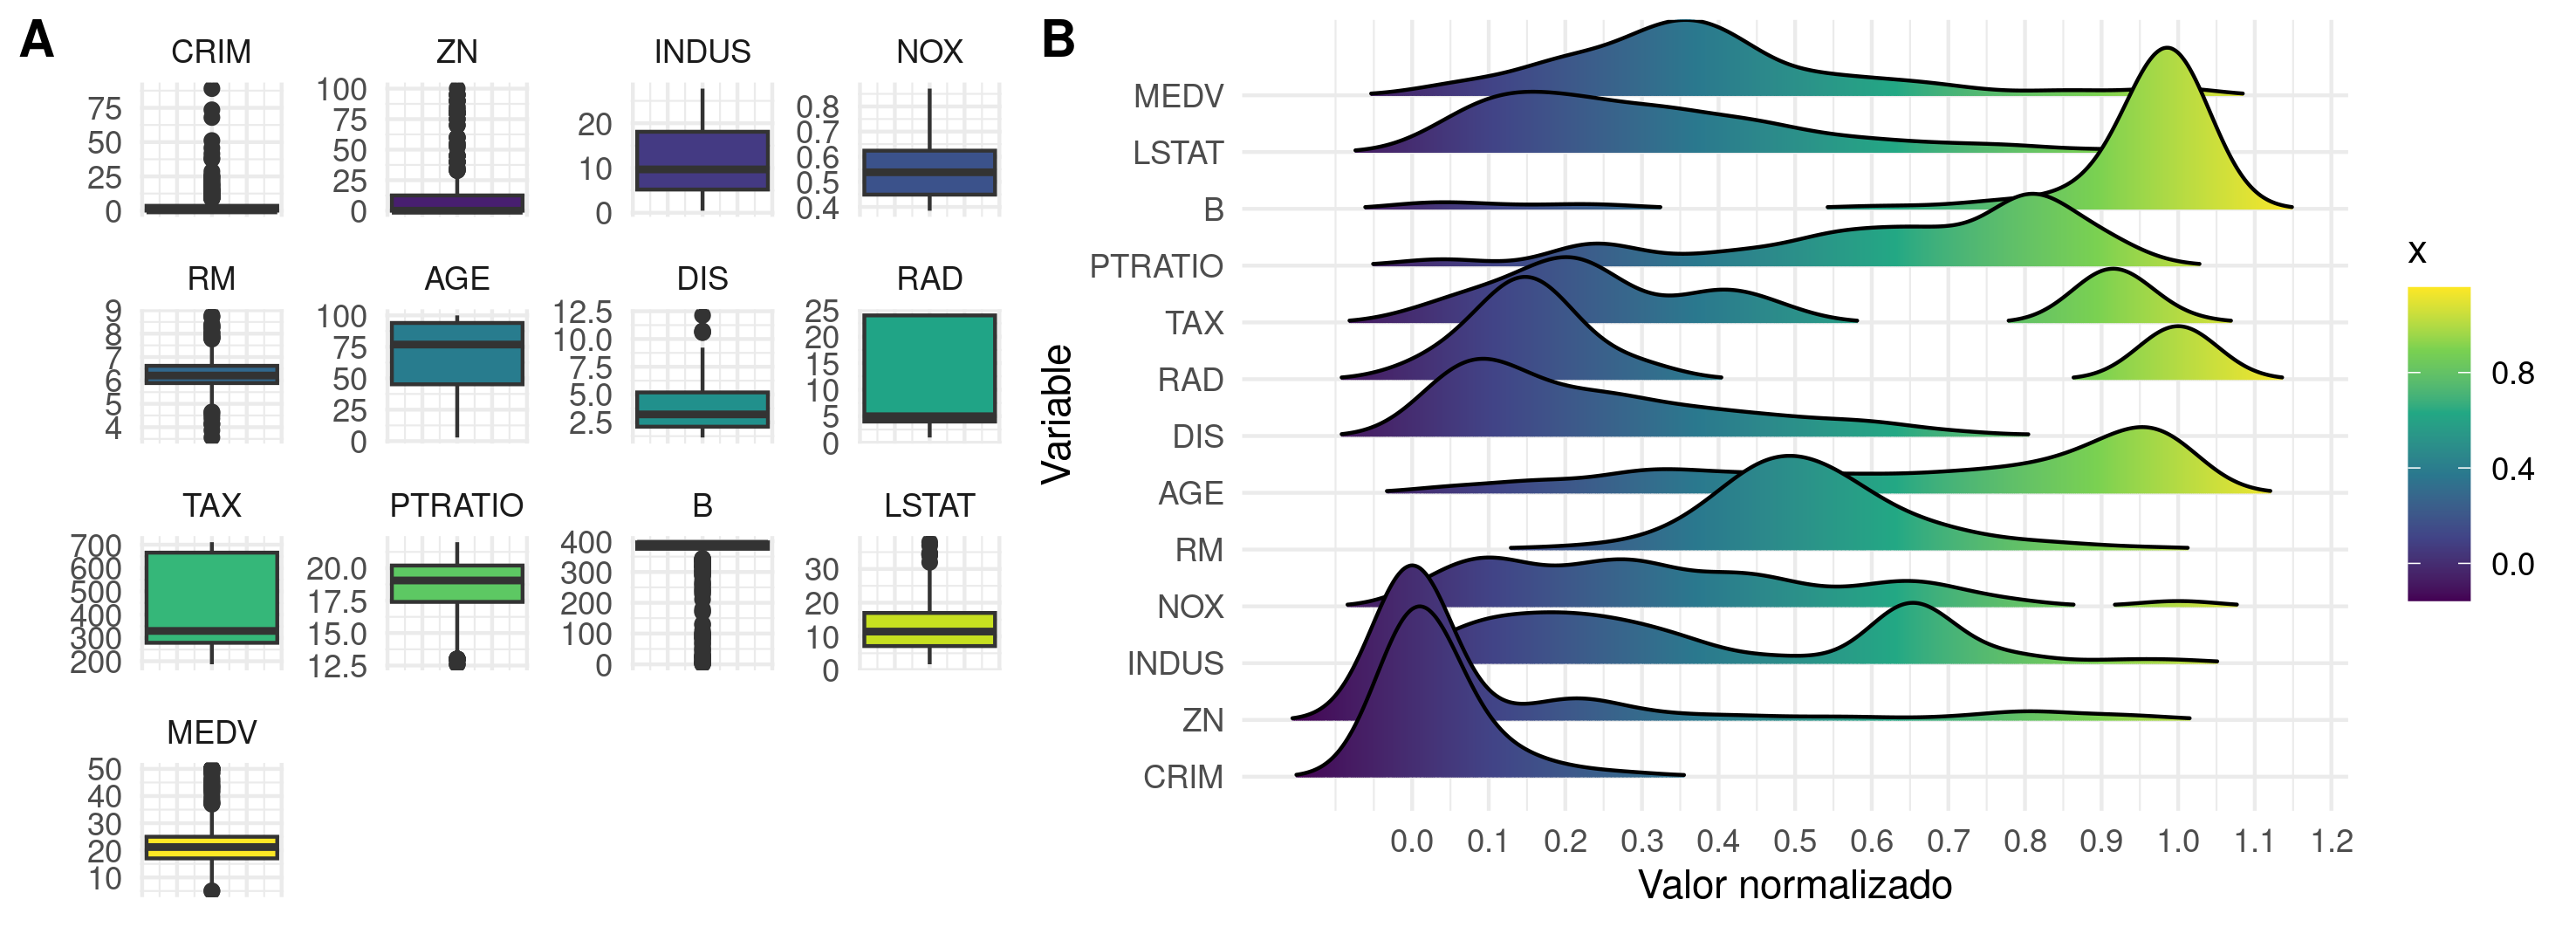
\includegraphics[width=0.95\textwidth]{figuras/boxplot-density.png}
	\caption{(A) Gráfico de cajas y bigotes de valores antes de normalización; (B) Gráfico de densidad después de normalización.}
	\label{fig:descriptive}
\end{figure}

Observando el gráfico de densidad (Figura \ref{fig:descriptive}(b)) también podemos ver que el número de cuartos por hogar (\codeword{RM}) está justamente a la mitad de sus datos normalizados, en $6.27\pm 0.70$ cuartos. Hay 64 residencias con un promedio mayor a 7 cuartos, y solamente 16 para mayores a 8 (Figura \ref{fig:histogram}), esto quiere decir que el 3.16\% de las residencias en Boston podrían considerarse de clase alta.

\begin{figure}[htb!]
	\centering
	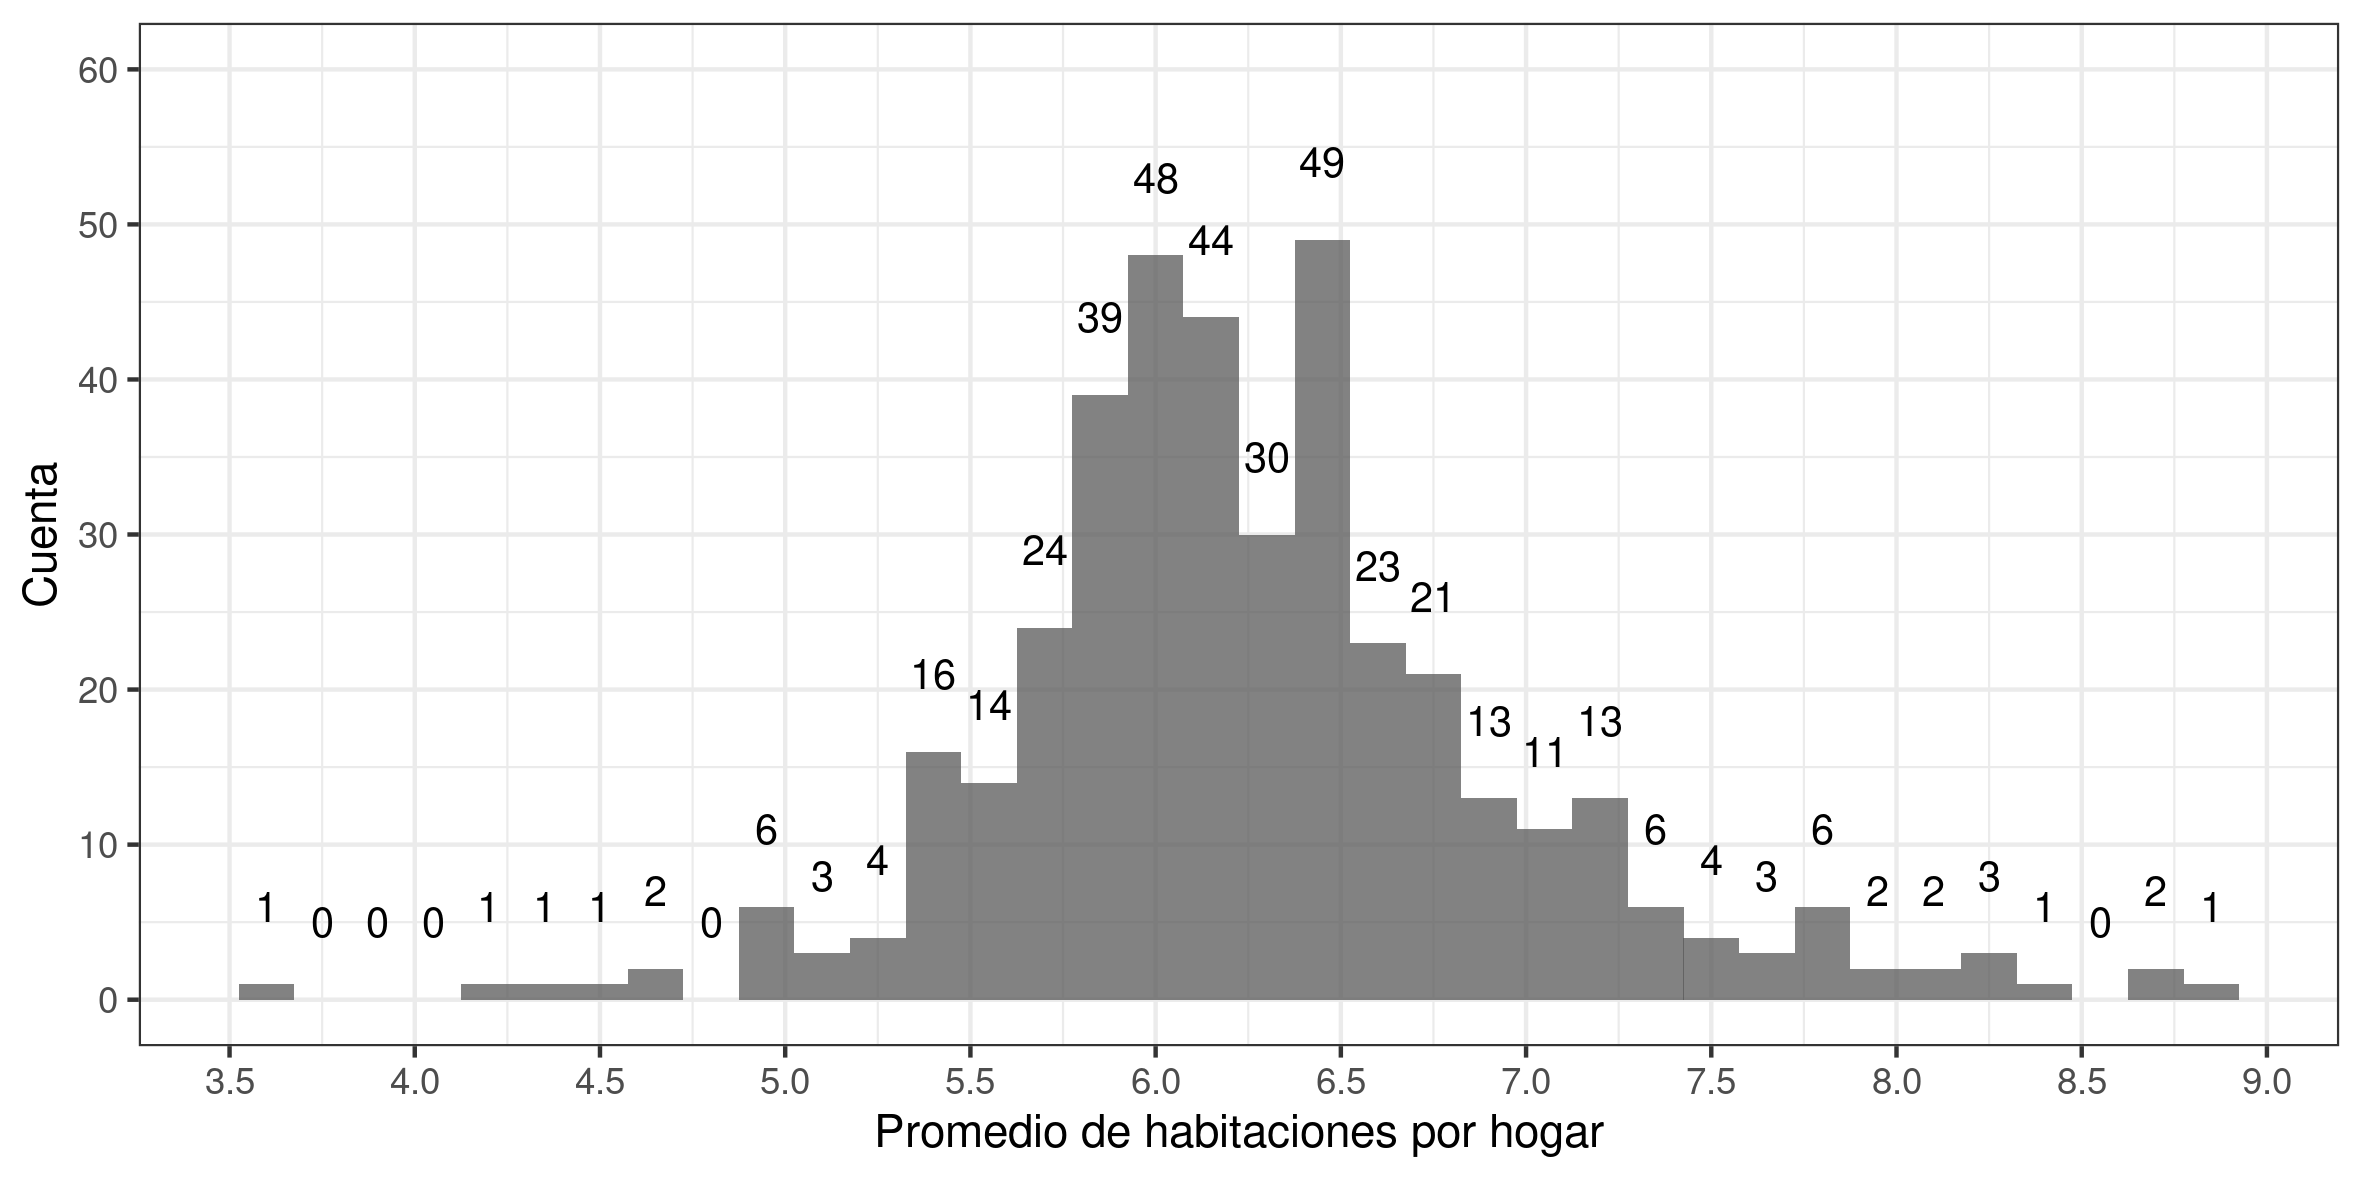
\includegraphics[width=0.75\textwidth]{figuras/RM-histogram.png}
	\caption{Histograma de cuenta para promedio de cuartos por residencia.}
	\label{fig:histogram}
\end{figure}

\subsection{Correlaciones}
Un cuadro de correlaciones (Figura \ref{fig:corrplot}) mostró que las variables \codeword{LSTAT} y \codeword{RM} tienen una alta relación con \codeword{MEDV}, esto va de acuerdo con los resultados de \codeword{Rank} y en los gráficos de dispersión (Figura \ref{fig:scatter}) se ve claramente una tendencia lineal. 

Estos resultados tienen sentido, ya que a medida que una casa con más cuartos costará más y menos es la cantidad de personas de clase baja que pueden pagarla.

\begin{figure}[htb!]
\begin{subfigure}[t]{0.35\textwidth}
	\centering
	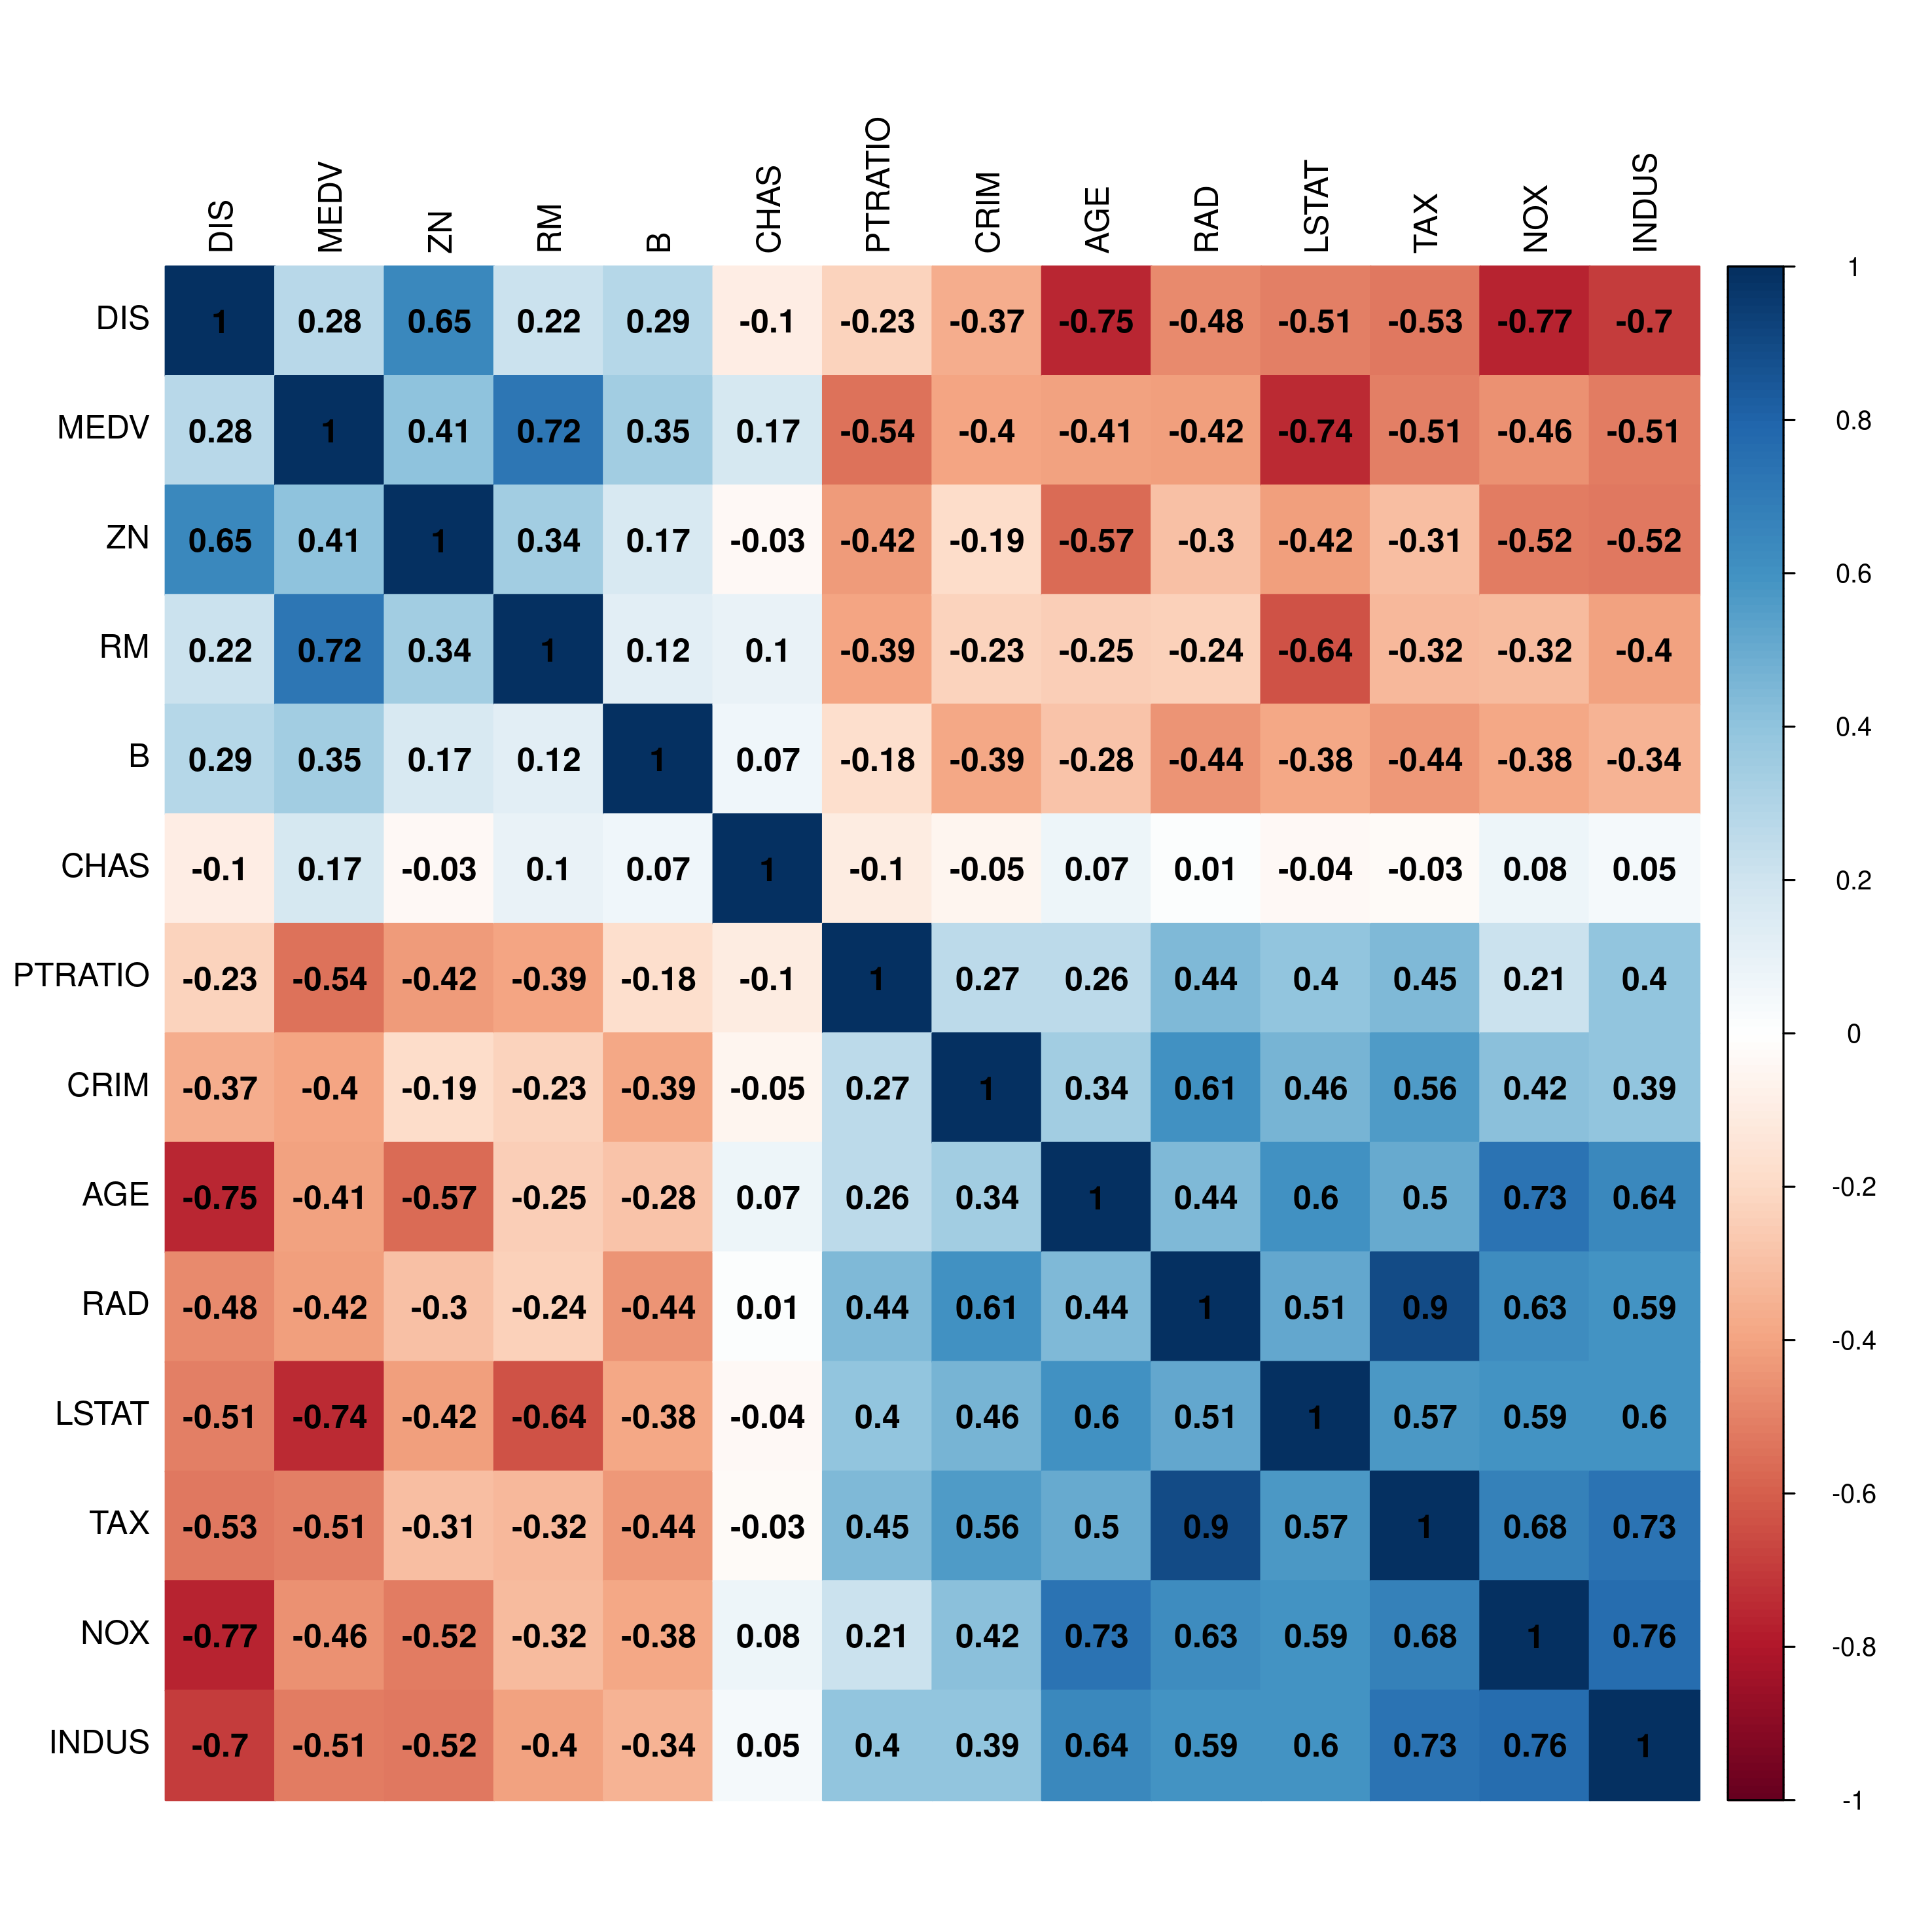
\includegraphics[width=0.95\textwidth]{figuras/corrplot.png}
	\caption{}
	\label{fig:corrplot}
\end{subfigure}
\hfill
\begin{subfigure}[t]{0.65\textwidth}
	\centering
	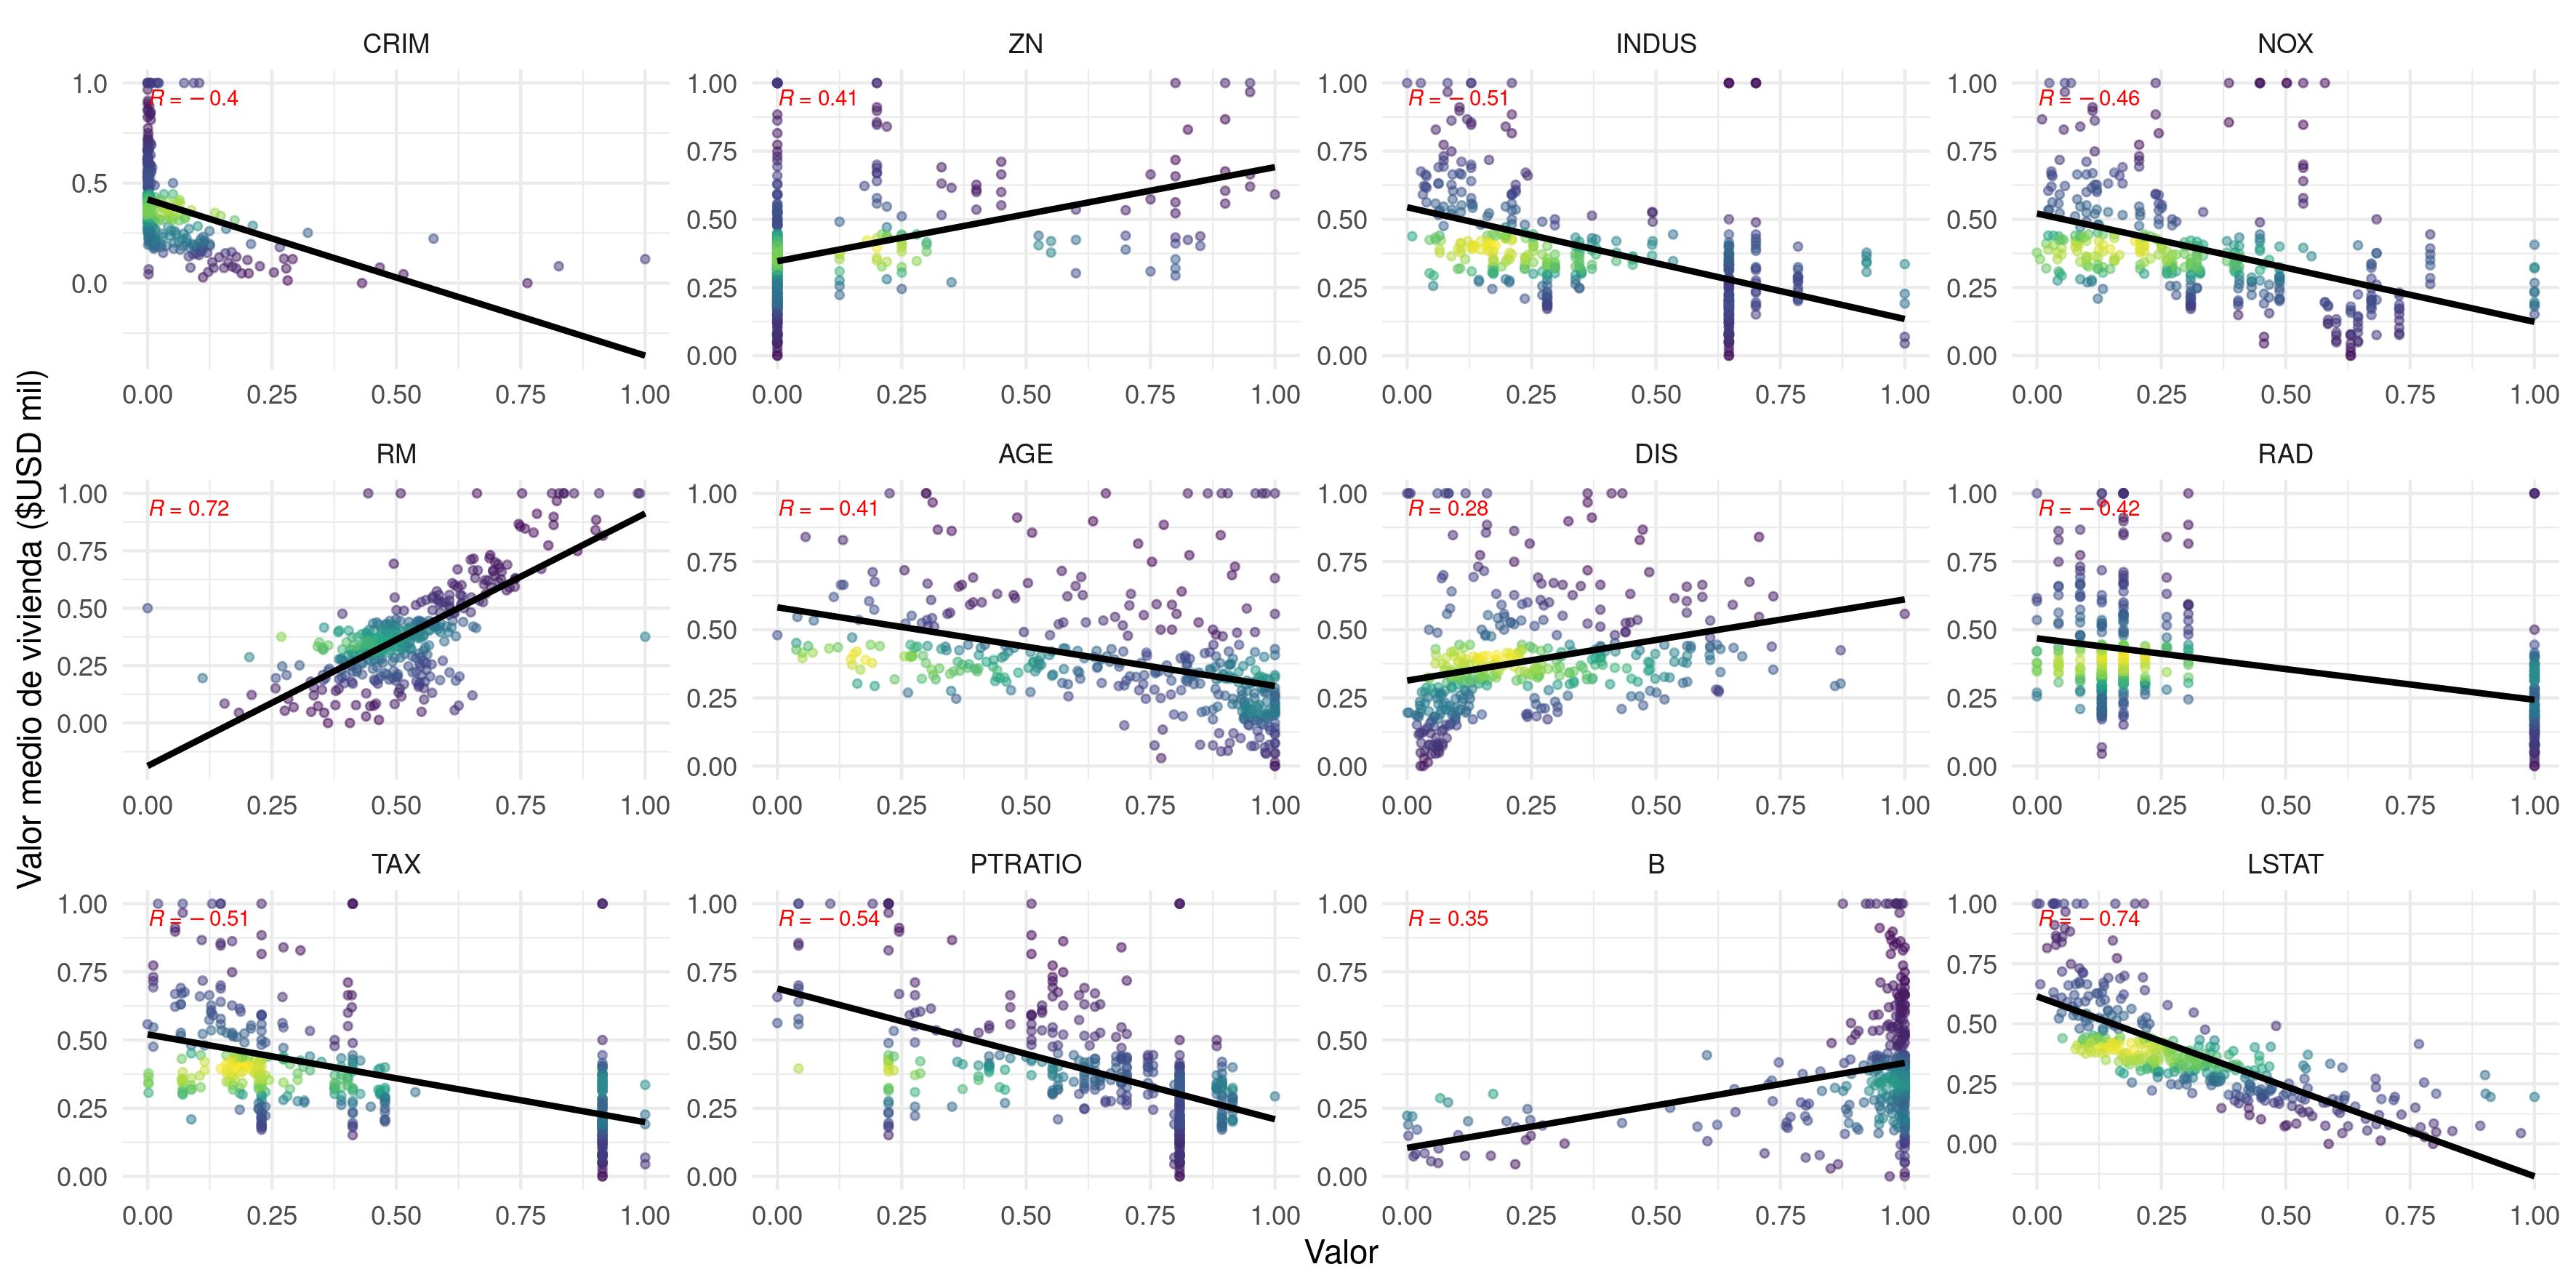
\includegraphics[width=0.90\textwidth]{figuras/scatter.png}
	\caption{}
	\label{fig:scatter}
\end{subfigure}
\caption{Gráficos descriptivos del modelo de Regresión Lineal Múltiple (RLM) (A) Matriz de correlación; (B) Gráfica de dispersión de todas las características numéricas del conjunto de datos en función de MEDV.}
\label{fig:regresion_descriptiva}
\end{figure}

En el mismo cuadro podemos observar que también existe una relación entre \codeword{LSTAT}-\codeword{RM} (Figura \ref{fig:rm_lstat}), con esto y la información anterior podemos concluir que a mayor número de cuartos, mayor será el costo de vivienda, por lo que una menor cantidad de personas de clase baja podrá pagar una de estas casas.

\begin{figure}
\centering
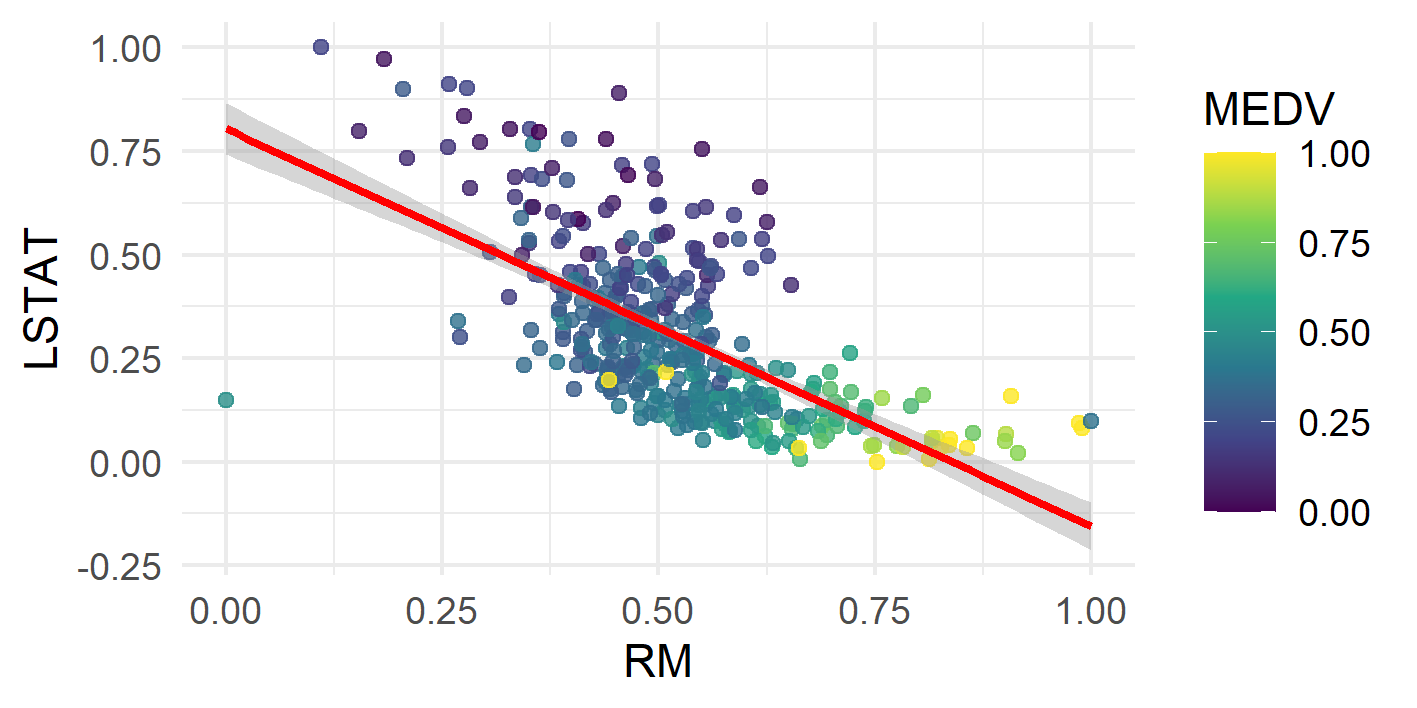
\includegraphics[width=0.5\textwidth]{figuras/rm_lstat.png}
\caption{Relación normalizada entre el promedio de habitaciones con el porcentaje de población de bajos recursos.}
\label{fig:rm_lstat}
\end{figure}

Sobre las demás variables que fueron seleccionadas con \codeword{Rank}, las correlaciones según la matriz no superaron el valor de $\pm 0.5$, así que podemos predecir que no se tomarán en cuenta para el modelo posteriormente.

Hay buenas correlaciones con la tasa de criminalidad per capita (\codeword{CRIM}) con algunas variables (ver Cuadro \ref{tab:variables}), como el índice de accesibilidad a carreteras radiales (\codeword{RAD}, corr=0.61) y la tasa de impuesto (\codeword{TAX}, corr=0.56), pero, a pesar de ser buenos resultados, no tienen ninguna relación entre sí.

\subsection{Regresión Lineal Múltiple}
A continuación se muestran los resultados presentados por el widget de \codeword{Test & Score} utilizando distintas combinaciones de parámetros, como \textit{Best Subset Selection} usando el 70\% de los datos como método de entrenamiento. Primero haciendo una regresión lineal para cada parámetro ($n=1$) en función de \codeword{MEDV}, y después usando todas ($n=13$). Finalmente se corrieron 4 combinaciones distintas para $n = \{2,3,4\}$ variables, dando un total de 26 combinaciones diferentes, ver Cuadro \ref{tab:testscore}.

Se utilizó el método de \textit{Best Subset Selection}\footnote{Se realizó de forma independiente del proyecto en \textit{R} con el paquete \textit{olss} con el único fin de presentar la gráfica de la Figura \ref{fig:bss}.} para encontrar la combinación de variables que mejor describieran al modelo. Los incrementos de $\mathrm{R}^2$ a partir de 4 parámetros fueron menores a 0.1, por lo que es seguro asumir que este es el número de variables necesarias para predecir el modelo. Haciendo referencia en el Cuadro \ref{tab:testscore} vemos que esa combinación de variables fueron \codeword{RM}+\codeword{PTRATIO}+\codeword{B}+\codeword{LSTAT} (ID = 22). 

\begin{figure}[h!]
	\centering
	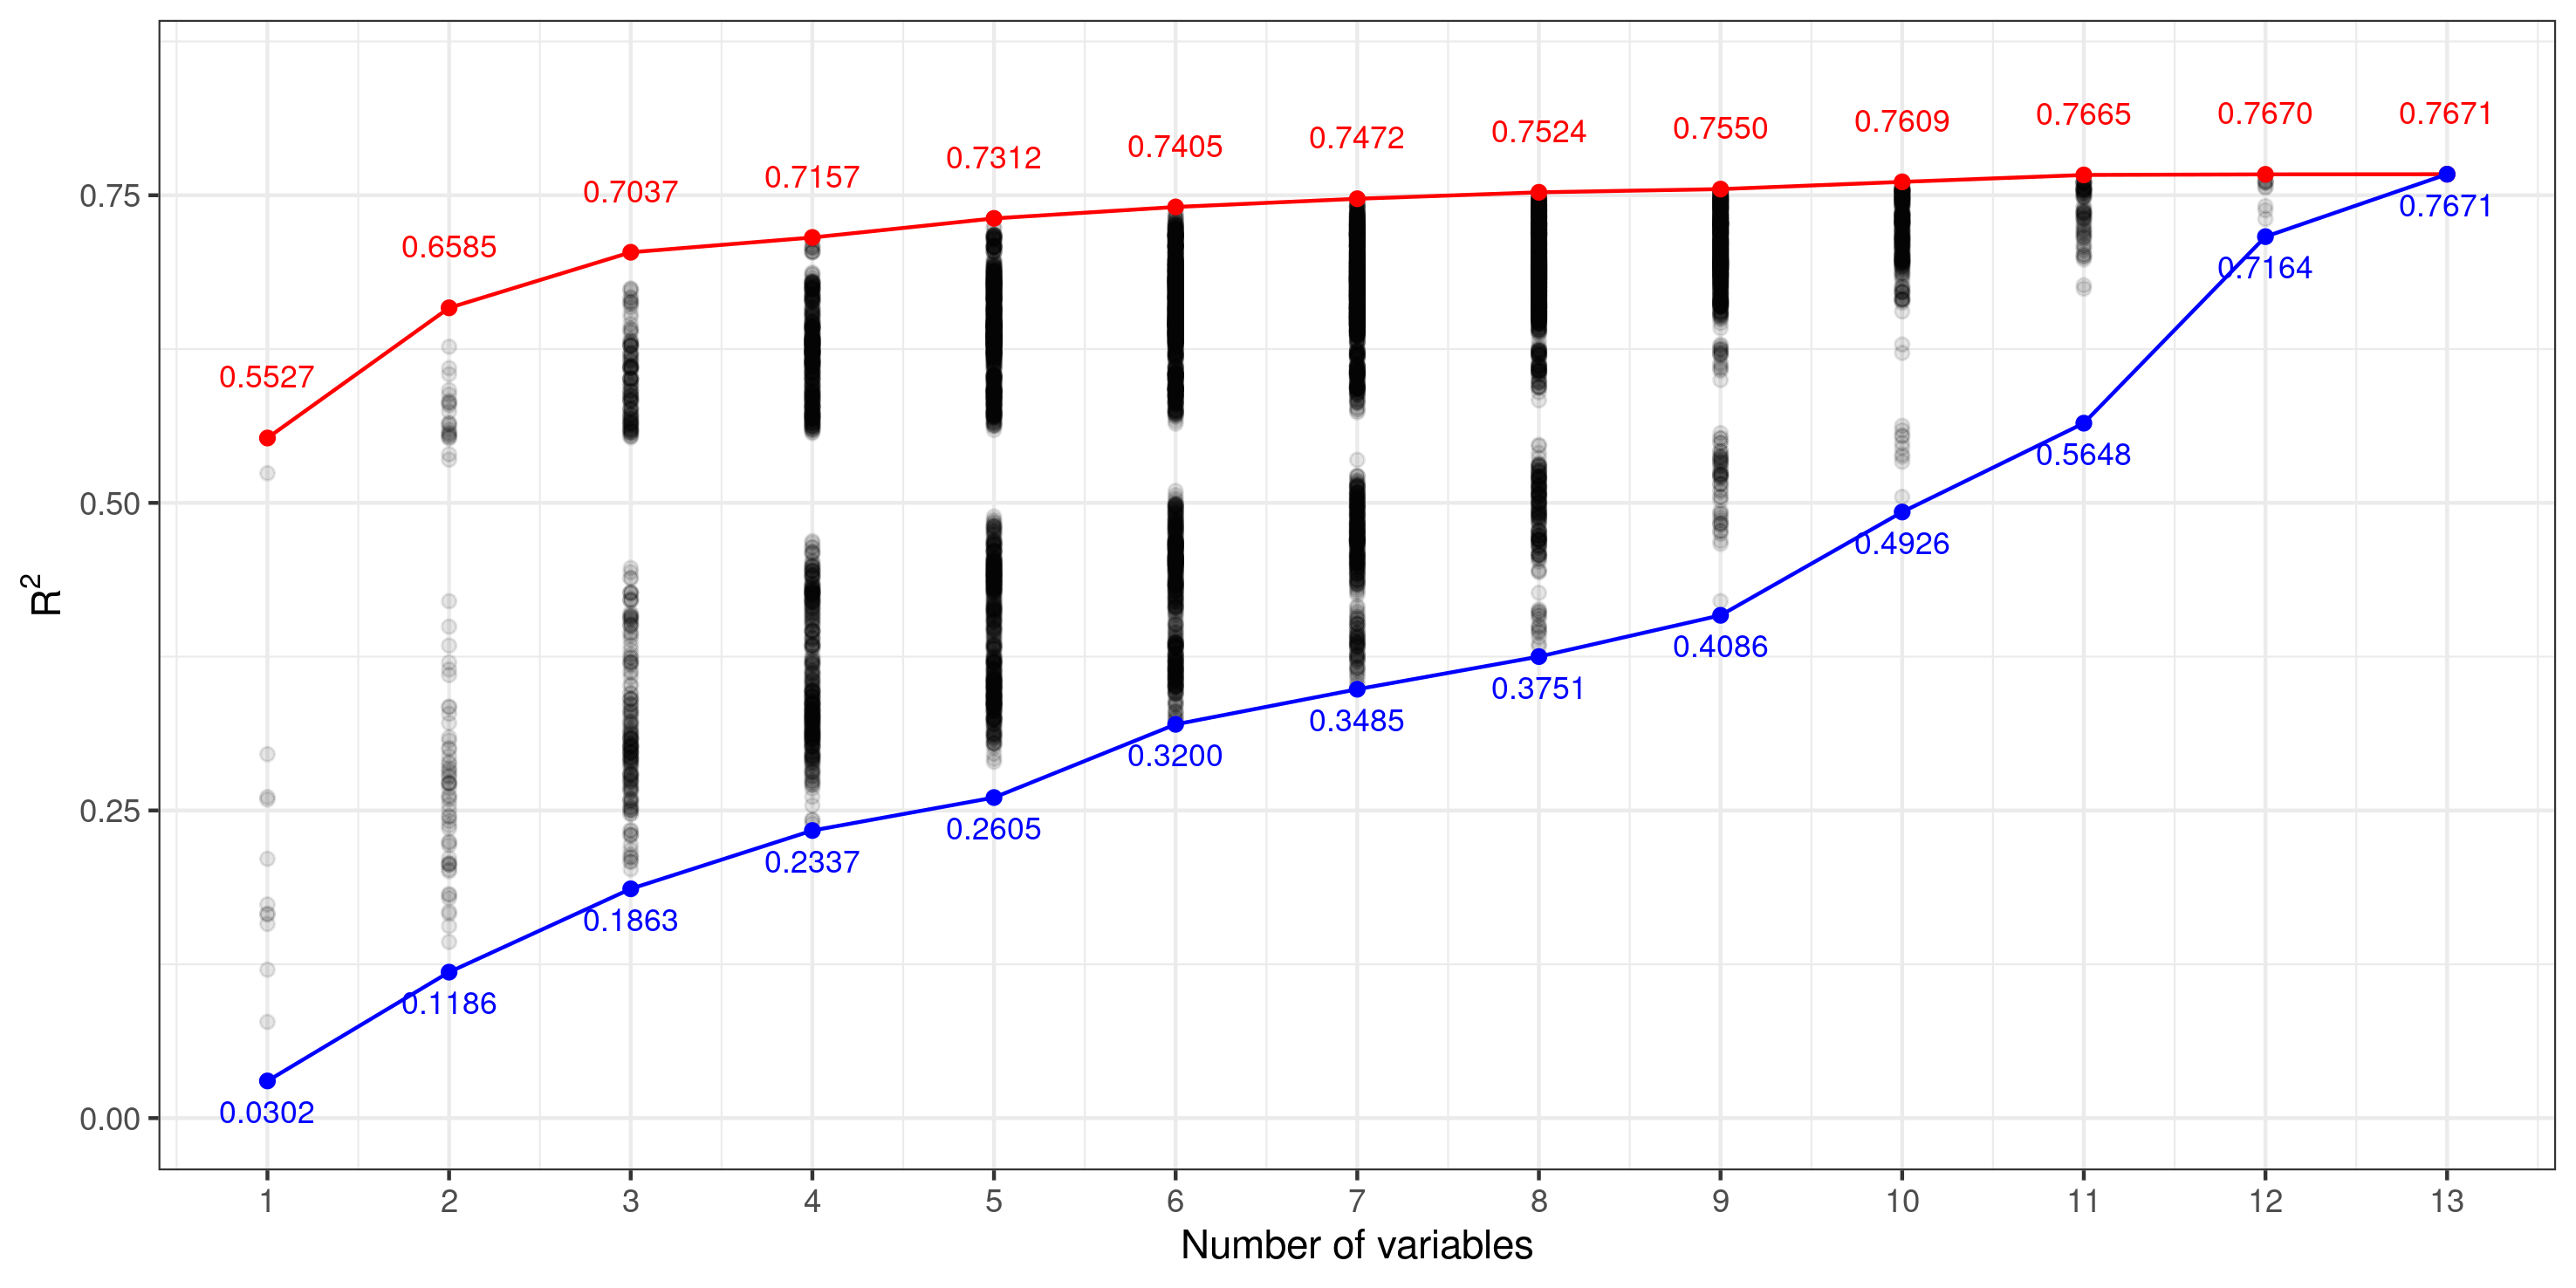
\includegraphics[width=0.9\textwidth]{figuras/best subset selection.png}
	\caption{Best Subset Selection (BSS) de todas las variables en \textit{Boston Housing}.}
	\label{fig:bss}
\end{figure}

Vemos que \codeword{LSTAT} y \codeword{RM} están presentes en la combinación, esto va a acorde con lo que se vió en el cuadro de correlaciones (Figura \ref{fig:corrplot}) y las tendencias en el gráfico de dispersión (Figura \ref{fig:scatter}), esto tiene sentido puesto que son variables que tienen una alta correlación con \codeword{MEDV}. La correlación negativa con \codeword{PTRATIO} indica que estas residencias se encuentran cerca de escuelas con una mayor cantidad de alumnos que de profesores; podríamos deducir que se trata de escuelas públicas donde existe una alta demanda de estudiantes y poca oferta de personal académico. Sobre la variable \codeword{B}, dado el contexto, parece ser solamente un parámetro \textit{circunstancial}, ya que---como se mencionó anteriormente---la mayoría de la población en todas las ciudades es negra, es decir, que las casas de alto valor como de bajo valor están ocupadas por esta población.

\section{Conclusiones}
La regresión lineal es una herramienta de \textit{statistical learning} sumamente útil para mostrar la relación de variables numéricas entre sí, y nos ayuda a poder formar una narrativa que nos ayude a explicar diversos fenómenos a partir de sus resultados.

En este proyecto se utilizó el software de \codeword{Orange} para jugar con los 13 parámetros del conjunto de datos de \textit{Boston Housing} para encontrar la mejor combinación que conteste la pregunta: ¿Qué es lo que afecta el valor mediano de hogares en Boston, MA?

De acuerdo con un Best Subset Selection manual, una regresión lineal múltiple que toma en cuenta todas las variables es el modelo que mejor describe el comportamiento de \codeword{MEDV}, sin embargo, solamente 4 a 6 variables son necesarias para describirlo. El precio medio de vivienda en Boston está dictado principalmente por el tamaño de la casa (\codeword{RM}) y, a su vez, existe una relación directa con el estrato social que tiene acceso a pagarlas (\codeword{LSTAT}). Las casas con menor valor son las que se encuentran en zonas con una baja proporción de alumno-maestro (\codeword{PTRATIO}), y las personas negras (\codeword{B}) tienen acceso a casas de alto valor como de bajo valor.

\printbibliography

\newpage
\appendix
\section{Descripción de variables}

\begin{table}[h!]
\centering
\begin{adjustbox}{width=\textwidth}
\begin{tabular}{llll}
\hline
\textbf{ID} & \textbf{Parámetro} & {\color[HTML]{000000} \textbf{Tipo de variable}} & \textbf{Descripción.}                                                                 \\ \hline
1           & CRIM               & {\color[HTML]{FE0000} Numérica}                  & Tasa de crimen \textit{per capita} por ciudad.                                                 \\
2           & ZN                 & {\color[HTML]{FE0000} Numérica}                  & Proporción de áreas residenciales con lotes mayores a 25mil $\mathrm{ft}^2$.          \\
3           & INDUS              & {\color[HTML]{FE0000} Numérica}                  & Proporción de acres comerciales no minoristas por ciudad.                             \\
4           & CHAS               & {\color[HTML]{FE0000} Numérica} / {\color[HTML]{32CB00} Categórica}     & Variable artificial del Río Charles (0 = No limita; 1 = Limita).                      \\
5           & NOX                & {\color[HTML]{FE0000} Numérica}                  & Concentración de óxidos nítricos (partes por 10millones).                             \\
6           & RM                 & {\color[HTML]{FE0000} Numérica}                  & Número promedio de habitaciones por vivienda.                                         \\
7           & AGE                & {\color[HTML]{FE0000} Numérica}                  & Proporción de unidades habitadas construidas antes de 1940.                           \\
8           & DIS                & {\color[HTML]{FE0000} Numérica}                  & Distancias ponderadas de 5 centros de empleo en Boston.                               \\
9           & RAD                & {\color[HTML]{FE0000} Numérica}                  & Índice de accesibilidad a carreteras radiales.                                        \\
10          & TAX                & {\color[HTML]{FE0000} Numérica}                  & Tasa de impuestos de propiedad completa por \$10,000 USD.                             \\
11          & PTRATIO            & {\color[HTML]{FE0000} Numérica}                  & Proporción alumno-maestro por ciudad.                                                 \\
12          & B                  & {\color[HTML]{FE0000} Numérica}                  & $1000(B_k - 0.63)^2$; donde $B_k$ es la proporción de población negra en   la ciudad. \\
13          & LSTAT              & {\color[HTML]{FE0000} Numérica}                  & Percentaje de personas que pertenecen a la clase baja en la ciudad.                   \\
14          & MEDV               & {\color[HTML]{FE0000} Numérica}                  & Valor mediano de propiedad ocupada en miles de USD (\$USDmil).                        \\ \hline
\end{tabular}
\end{adjustbox}
\caption{Tabla de descripción de variables en el conjunto de datos \textit{Boston Housing}.}
\label{tab:variables}
\end{table}

\section{Tablas de resultados}

\begin{table}[h!] % Tabla de resultados de Best Subset Selections
\centering
\begin{adjustbox}{width=\textwidth}
\begin{tabular}{lllllll}
\hline
\textbf{ID} & \textbf{n} & \textbf{Predictores}                                      & \textbf{MSE} & \textbf{RMSE} & \textbf{MAE} & \textbf{$\mathrm{R}^2$} \\ \hline
1           & 1          & LSTAT                                                     & 40.4230      & 6.3580        & 4.5910       & 0.5527         \\
2           & 1          & RM                                                        & 46.0536      & 6.7863        & 4.5399       & 0.5241         \\
3           & 1          & PTRATIO                                                   & 66.9565      & 8.1827        & 5.9830       & 0.2957         \\
4           & 1          & INDUS                                                     & 72.1585      & 8.4946        & 6.0492       & 0.2609         \\
5           & 1          & TAX                                                       & 65.3017      & 8.0809        & 5.7910       & 0.2589         \\
6           & 1          & NOX                                                       & 68.3234      & 8.2658        & 5.9955       & 0.2107         \\
7           & 1          & RAD                                                       & 73.6673      & 8.5830        & 6.1894       & 0.1736         \\
8           & 1          & AGE                                                       & 67.8550      & 8.2374        & 5.6922       & 0.1660         \\
9           & 1          & ZN                                                        & 70.5212      & 8.3977        & 5.9814       & 0.1655         \\
10          & 1          & CRIM                                                      & 70.6842      & 8.4074        & 6.0218       & 0.1578         \\
11          & 1          & B                                                         & 76.9584      & 8.7726        & 6.2886       & 0.1206         \\
12          & 1          & DIS                                                       & 79.9044      & 8.9389        & 6.3977       & 0.0781         \\
13          & 1          & CHAS                                                      & 82.2370      & 9.0685        & 6.7172       & 0.0302         \\
14          & 2          & RM LSTAT                                                  & 33.3145      & 5.7719        & 4.1470       & 0.6585         \\
15          & 2          & PTRATIO LSTAT                                             & 36.2053      & 6.0171        & 4.2816       & 0.6269         \\
16          & 2          & RM TAX                                                    & 38.7602      & 6.2258        & 4.0774       & 0.6095         \\
17          & 2          & RM PTRATIO                                                & 40.3046      & 6.3486        & 4.2659       & 0.6045         \\
18          & 3          & RM PTRATIO LSTAT                                          & 30.6197      & 5.5335        & 3.9051       & 0.7037         \\
19          & 3          & RM TAX LSTAT                                              & 33.3924      & 5.7786        & 4.0956       & 0.6740         \\
20          & 3          & RM B LSTAT                                                & 32.4562      & 5.6970        & 4.0444       & 0.6739         \\
21          & 3          & CHAS RM LSTAT                                             & 29.3583      & 5.4183        & 3.8614       & 0.6721         \\
22          & 4          & RM PTRATIO B LSTAT                                        & 30.0252      & 5.4795        & 3.7939       & 0.7157         \\
23          & 4          & CHAS RM PTRATIO LSTAT                                     & 24.6675      & 4.9666        & 3.4114       & 0.7135         \\
24          & 4          & RM DIS PTRATIO LSTAT                                      & 29.8113      & 5.4600        & 3.8567       & 0.7095         \\
25          & 4          & CRIM RM PTRATIO LSTAT                                     & 22.8367      & 4.7788        & 3.3647       & 0.7082         \\
26          & 13         & CRIM ZN INDUS CHAS NOX RM AGE DIS RAD TAX PTRATIO B LSTAT & 24.5508      & 4.9549        & 3.4464       & 0.7671         \\ \hline
\end{tabular}
\end{adjustbox}
\caption{Resultados de \textit{Test \& Score} para distintas combinaciones de parámetros del conjunto de datos.}
\label{tab:testscore}
\end{table}

\end{document}
